\chapter{Biologie de la conservation}\label{ch:b3:conservation-biology}

En 1813 Audubon regarda pendant trois jours un vol de tourtes voyageuses
passer au-dessus du Kentucky en obscurcissant le ciel~; elles étaient
peut-être cinq milliards, le quart de tous les oiseaux d'Amérique du
Nord. Le 1\textsuperscript{er}~septembre 1914 la dernière, une femelle
nommée Martha, mourut au zoo de Cincinnati. L'espèce n'était pas rare
quand son déclin commença~; on la récoltait par wagons entiers, on
coupait ses forêts, et un oiseau qui ne se reproduisait qu'en colonies
immenses ne put plus se reproduire une fois les colonies raréfiées
au-dessous d'une taille que personne n'avait mesurée. En 1995 le
kakapo, perroquet nocturne et inapte au vol de Nouvelle-Zélande, n'était
plus qu'à cinquante et un oiseaux~; chacun a depuis été nommé, pesé,
équipé d'un émetteur et, au bon moment, gratifié d'un repas
supplémentaire, et ils sont deux cent cinquante. La même année trente et
un loups gris furent lâchés à Yellowstone, soixante-dix ans après que la
dernière meute native eut été abattue~; en deux décennies les wapitis
avaient bougé, les saules étaient revenus le long des rivières, et les
castors avec eux. La biologie de la conservation est l'application de la
génétique des populations, de l'écologie et du comportement de ce livre
à une seule question pratique --- comment empêcher les espèces de
disparaître --- et son arithmétique est celle des petits nombres.

\section{Pourquoi les petites populations meurent}

\begin{definition}[Les risques de la petitesse]\label{def:b3:conservation-biology:small}
\index{stochasticité démographique}\index{stochasticité environnementale}\index{effet Allee}\index{vortex d'extinction}\index{population minimale viable}
Une grande population décline quand son taux de mortalité dépasse son
taux de natalité~; une petite peut s'évanouir sans que ni l'un ni
l'autre change. La \emph{stochasticité démographique} est le hasard
qui fait que, parmi quelques individus, il en meurt plus qu'il n'en
naît, ou que tous les survivants sont des mâles~: elle compte au-dessous
de quelques dizaines. La \emph{stochasticité environnementale} --- un
mauvais hiver, une sécheresse, une maladie --- frappe tous les individus
à la fois, et une population de quelques centaines qu'une grande
encaisserait peut être anéantie~; les \emph{catastrophes} en sont la
queue de distribution. L'\emph{effet Allee} fait baisser le taux de
croissance par tête à faible densité --- on ne trouve pas de partenaire,
les nicheurs coloniaux ne peuvent nicher, les hardes ne peuvent défendre
leurs jeunes, les vols de tourtes voyageuses ne pouvaient plus saturer
les prédateurs qui prenaient leurs jeunes --- de sorte qu'au-dessous
d'une densité seuil la population décline d'elle-même vers zéro. Et
au-dessous de quelques centaines, les processus génétiques de la section
suivante abaissent la valeur sélective génération après génération. Tout
cela s'alimente~: une population plus petite perd de la variation,
devient moins féconde, rapetisse, est plus exposée au hasard, et en perd
davantage --- le \emph{vortex d'extinction} (Gilpin et Soulé, 1986). Une
\emph{population minimale viable} est la taille au-dessus de laquelle la
probabilité d'extinction sur un horizon donné (disons \qty{5}{\%} en un
siècle) est acceptable~; elle dépend de la biologie de l'espèce et de la
variabilité de son environnement, et se compte d'ordinaire en milliers.
\end{definition}

\begin{omfigure}
\begin{tikzpicture}[every node/.style={font=\scriptsize}, >=stealth]
  \node[draw, thick, rounded corners, fill=omThm!20, align=center] (small) at (0,0) {la population\\devient petite};
  \node[draw, thick, rounded corners, fill=omDef!20, align=center] (drift) at (3.4,1.6) {dérive et consanguinité~:\\variation perdue, $F$ monte};
  \node[draw, thick, rounded corners, fill=omDef!20, align=center] (fit) at (6.8,0) {la valeur sélective baisse~:\\moins de jeunes, plus de maladies};
  \node[draw, thick, rounded corners, fill=omDef!20, align=center] (chance) at (3.4,-1.6) {les hasards démographique et\\environnemental mordent plus fort};
  \node[draw, thick, rounded corners, fill=omProp!25, align=center] (allee) at (9.9,0) {effet Allee~:\\croissance négative};
  \draw[->, very thick] (small) -- (drift); \draw[->, very thick] (drift) -- (fit); \draw[->, very thick] (fit) -- (chance); \draw[->, very thick] (chance) -- (small);
  \draw[->, thick, omProp!80!black] (fit) -- (allee); \draw[->, thick, omProp!80!black] (allee.south) .. controls (9.9,-3) and (0,-3.4) .. (small.south);
  \node[align=center, font=\tiny] at (3.4,0) {le vortex d'extinction~:\\chaque tour rétrécit la\\population et accélère le suivant};
  \node[left, align=right, font=\tiny] at (-1.7,1.5) {perte d'habitat, récolte,\\prédateurs envahissants,\\maladies~: la population\\est poussée vers le bas};
  \draw[->, thick, gray] (-1.6,1.2) -- (small.north west);
\end{tikzpicture}

{\small Le \omterm{def:b3:conservation-biology:small}{vortex d'extinction}. Un coup extérieur rend une population
petite~; la petitesse fait alors perdre de la variation, abaisse la
valeur sélective, expose la population au hasard, et la rend plus petite
encore. La tâche de la conservation est de rompre la boucle avant
qu'elle ne se referme.}
\end{omfigure}

\begin{theorem}[La taille efficace de population]\label{thm:b3:conservation-biology:ne}
\index{taille efficace de population}\index{sex-ratio}\index{moyenne harmonique}\index{coefficient de consanguinité}\index{hétérozygotie}
Le rythme auquel une population perd de la variation et accumule de la
consanguinité est gouverné non par son effectif de recensement $N$ mais
par sa \emph{taille efficace} $N_{e}$~: la taille d'une population
idéale --- constante, à panmixie, à sex-ratio équilibré, à tailles de
familles poissonniennes --- qui perdrait de l'hétérozygotie au même
rythme. Trois écarts à l'idéal l'abaissent. Un sex-ratio déséquilibré,
avec $N_{m}$ mâles reproducteurs et $N_{f}$ femelles~:
\[
N_{e} = \frac{4N_{m}N_{f}}{N_{m} + N_{f}} ;
\]
un mâle et cent femelles donnent $N_{e} \approx 4$. Une taille qui
fluctue sur $t$ générations~: $N_{e}$ est la \emph{\omterm{thm:b3:conservation-biology:ne}{moyenne harmonique}}
des tailles de génération, $1/N_{e} = (1/t)\sum 1/N_{i}$, dominée par la
plus petite --- une population de mille qui est un jour passée par dix a
un $N_{e}$ voisin de cent sur cet intervalle. Et une variance des
tailles de familles supérieure à celle de Poisson l'abaisse encore. Dans
une population de taille efficace $N_{e}$ le \emph{\omterm{thm:b3:conservation-biology:ne}{coefficient de
consanguinité}} $F$ --- la probabilité que les deux allèles d'un locus
chez un individu soient les copies d'un même allèle ancestral --- monte
de $1/2N_{e}$ par génération,
\[
F_{t} = 1 - \Bigl(1 - \frac{1}{2N_{e}}\Bigr)^{t} \approx \frac{t}{2N_{e}},
\qquad H_{t} = H_{0}\Bigl(1 - \frac{1}{2N_{e}}\Bigr)^{t} ,
\]
et l'\emph{hétérozygotie} $H$ décroît au même rythme. La règle empirique
de Franklin, «~50/500~»~: $N_{e} \ge 50$ tient la consanguinité
au-dessous de \qty{1}{\%} par génération, le rythme que tolèrent les
éleveurs~; $N_{e} \ge
500$ permet à la mutation de remplacer la variation que la dérive
retire. Comme $N_{e}$ vaut d'ordinaire le dixième de l'effectif
recensé, la règle réclame des populations de cinq cents à cinq mille.
\end{theorem}
\begin{proof}
Deux gamètes tirés au hasard dans la population sont copies du même
allèle parental avec la probabilité $1/2N$ dans la population idéale, ce
qui est l'incrément de $F$~; l'hétérozygotie vaut $1 - F$ à un facteur
près, de sorte que chaque génération la multiplie par $(1 - 1/2N_{e})$,
d'où la décroissance exponentielle et, pour $t \ll N_{e}$, la montée
linéaire de $F$. Le sex-ratio~: la moitié des gènes vient de chaque
sexe, de sorte que la chance que deux gamètes partagent un allèle
parental vaut $\tfrac{1}{4}\cdot\tfrac{1}{2N_{m}} +
\tfrac{1}{4}\cdot\tfrac{1}{2N_{f}}$ (un quart des paires sont toutes
deux paternelles, un quart toutes deux maternelles)~; en égalant cela à
$1/2N_{e}$ on obtient $1/N_{e} = 1/(4N_{m}) + 1/(4N_{f})$, la formule.
La fluctuation~: l'hétérozygotie après $t$ générations vaut
$H_{0}\prod(1 - 1/2N_{i})
\approx H_{0}\exp(-\sum 1/2N_{i})$, égale à $H_{0}\exp(-t/2N_{e})$ quand
$1/N_{e}$ est la moyenne des $1/N_{i}$. La consanguinité abaisse la
valeur sélective parce qu'elle expose à l'état homozygote des allèles
récessifs délétères --- la \emph{dépression de consanguinité}, une chute
de plusieurs pour cent de la survie ou de la fécondité par tranche de
\qty{10}{\%} de $F$ chez la plupart des espèces allogames.
\end{proof}

\begin{omfigure}
\begin{tikzpicture}
\begin{axis}[
  width=0.46\linewidth, height=5.2cm,
  axis x line=bottom, axis y line=left,
  xmin=0, xmax=1, ymin=0, ymax=1.05,
  xlabel={fraction de mâles parmi les reproducteurs}, ylabel={$N_{e}/N$},
  xlabel style={font=\small, at={(axis description cs:0.5,-0.12)}, anchor=north}, ylabel style={font=\small},
  tick label style={font=\small}, xtick={0,0.1,0.5,0.9,1}, ytick={0.36,1},
  clip=false,
]
\addplot[very thick, omDef, domain=0.005:0.995, samples=100] {4*x*(1-x)};
\draw[dashed, gray] (axis cs:0.1,0) -- (axis cs:0.1,0.36) -- (axis cs:0,0.36);
\node[font=\scriptsize, omDef, anchor=south] at (axis cs:0.5,1.0) {sexes équilibrés~: $N_{e} = N$};
\node[font=\scriptsize, anchor=west, align=left] at (axis cs:0.12,0.2) {un mâle sur dix\\reproducteur~: $N_{e} = 0.36N$};
\end{axis}
\begin{axis}[
  at={(0.5\linewidth,0)}, anchor=south west,
  width=0.46\linewidth, height=5.2cm,
  axis x line=bottom, axis y line=left,
  xmin=0, xmax=100, ymin=0, ymax=1.05,
  xlabel={générations}, ylabel={hétérozygotie $H_{t}/H_{0}$},
  xlabel style={font=\small, at={(axis description cs:0.5,-0.12)}, anchor=north}, ylabel style={font=\small},
  tick label style={font=\small}, xtick={0,25,50,75,100}, ytick={0.37,0.6,0.9,1},
  yticklabels={0.37,0.6,0.9,1},
  clip=false,
]
\addplot[very thick, omThm, domain=0:100, samples=60] {(1-1/20)^x};
\addplot[very thick, omMeth!70!black, domain=0:100, samples=60] {(1-1/100)^x};
\addplot[very thick, omDef, domain=0:100, samples=60] {(1-1/1000)^x};
\node[font=\scriptsize, omThm, anchor=north west] at (axis cs:12,0.55) {$N_{e} = 10$};
\node[font=\scriptsize, omMeth!70!black, anchor=south west] at (axis cs:50,0.62) {$N_{e} = 50$};
\node[font=\scriptsize, omDef, anchor=south west] at (axis cs:60,0.95) {$N_{e} = 500$};
\end{axis}
\end{tikzpicture}

{\small À gauche~: comment un sex-ratio déséquilibré rétrécit la taille
efficace --- une espèce à harem dont un dixième des mâles se reproduit a
un $N_{e}$ égal au tiers de son effectif recensé. À droite~:
l'hétérozygotie décroissant de $(1 - 1/2N_{e})$ par génération --- une
population de dix perd l'essentiel de sa variation en un siècle, une de
cinq cents presque rien.}
\end{omfigure}

\begin{proof}[Faits expérimentaux]
La panthère de Floride, tombée à quelque vingt-cinq animaux dans les
années 1990, montrait des queues coudées, des testicules non descendus,
des malformations cardiaques et un sperme anormal à \qty{90}{\%} --- une
dépression de consanguinité rendue visible~; huit femelles introduites
du Texas en 1995 (un \emph{sauvetage génétique}) ont triplé la
population et les défauts ont reculé. Les loups de l'île Royale, fondés
par un couple en 1949 et isolés, ont décliné jusqu'à deux individus
grossièrement consanguins en 2018, avec des déformations vertébrales sur
la plupart des squelettes examinés. Le tétras cupidon de l'Illinois est
tombé de milliers à cinquante, et son taux d'éclosion de \qty{93}{\%} à
\qty{56}{\%}, avant de se rétablir après l'apport d'oiseaux d'autres
États. Les peaux de musée et l'ADN ancien permettent de mesurer
directement la perte d'hétérozygotie face à la population d'avant le
déclin dans chacun de ces cas.
\end{proof}

\begin{omfigure}
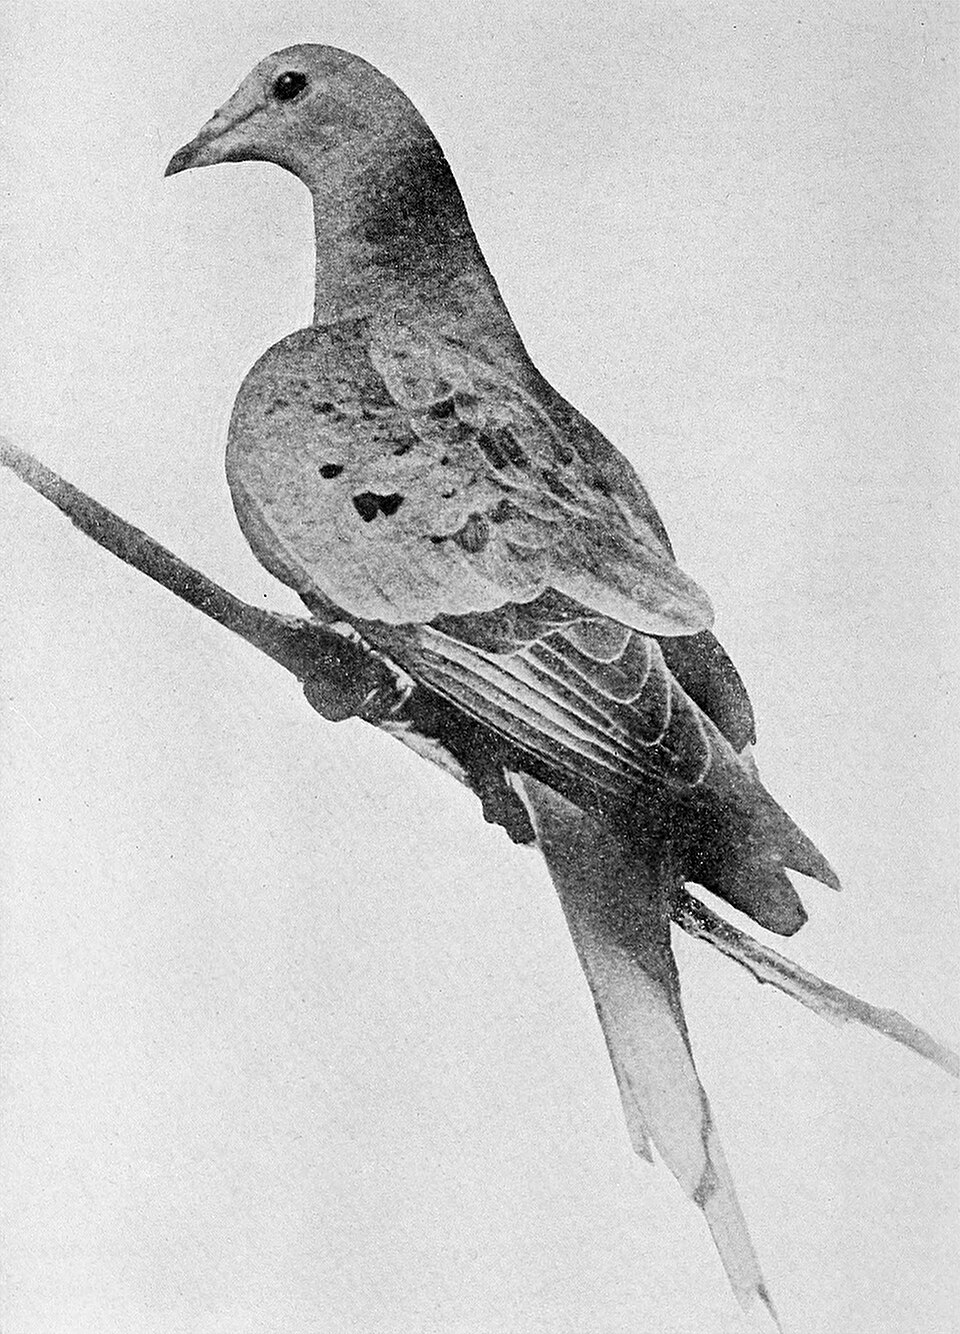
\includegraphics[width=0.4\linewidth]{images/book5/martha.jpg}\hspace{0.04\linewidth}
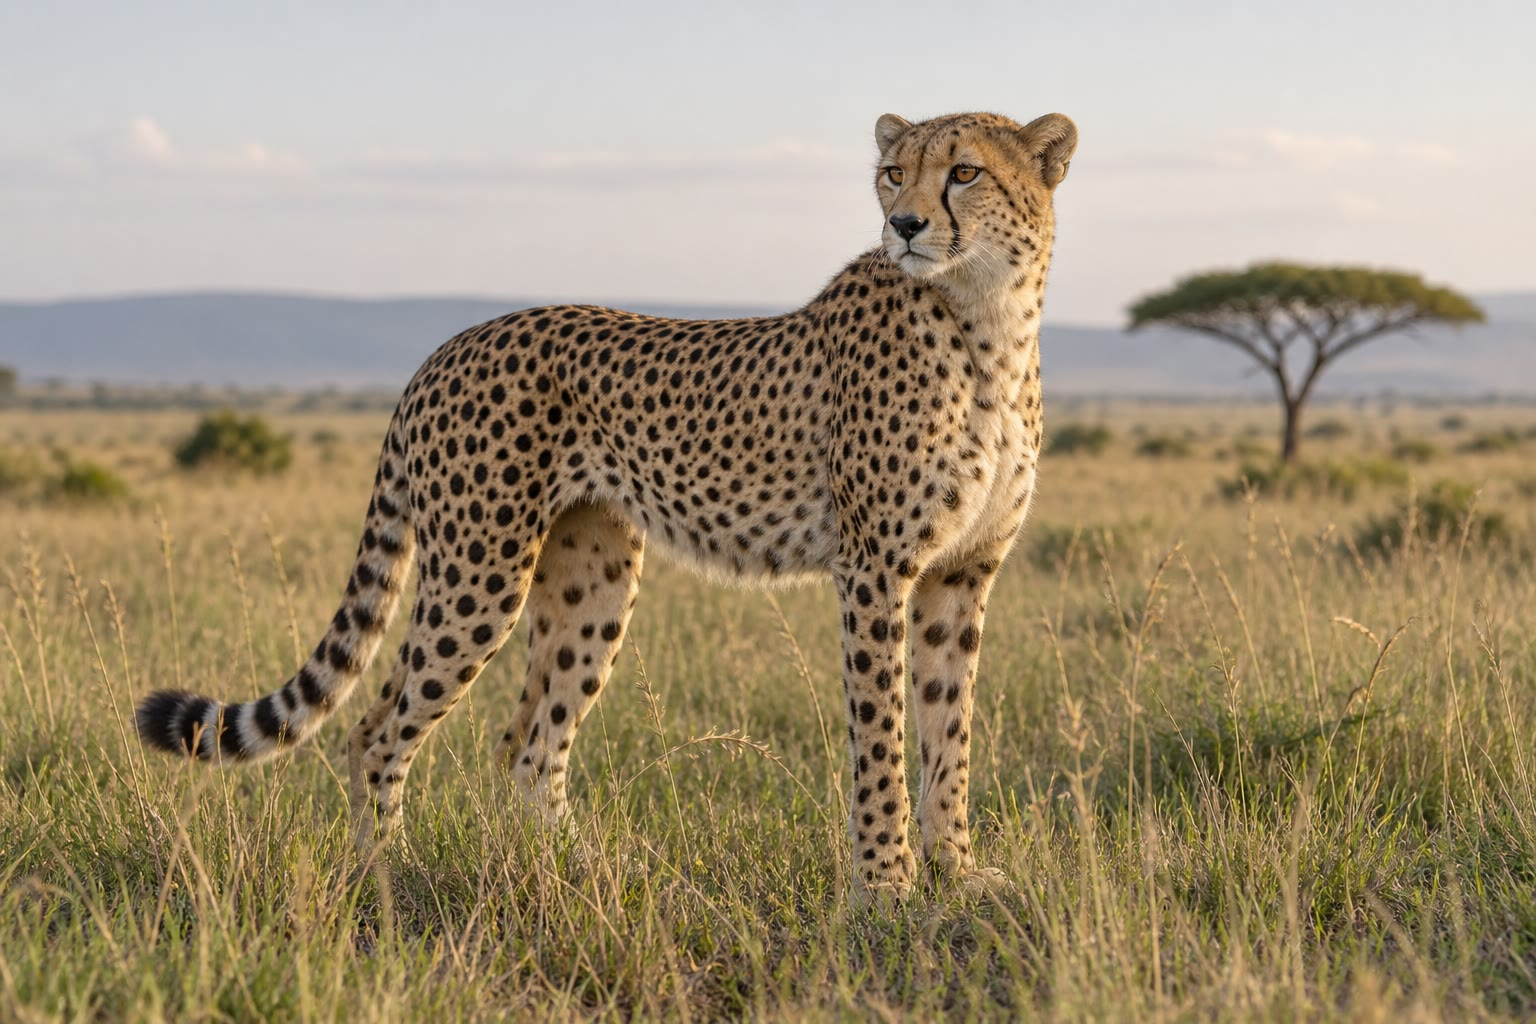
\includegraphics[width=0.52\linewidth]{images/book5/ai/b5-27-cheetah.jpg}

{\small À gauche~: Martha, la dernière tourte voyageuse, photographiée au
zoo de Cincinnati en 1912~; l'espèce se comptait en milliards de mémoire
d'homme (photographie d'Enno Meyer, domaine public). À droite~: un
guépard --- une espèce passée par un goulot d'étranglement il y a une
dizaine de milliers d'années et dont les individus se ressemblent tant
que les greffes de peau entre animaux non apparentés ne sont pas
rejetées.}
\end{omfigure}

\section{L'habitat~: quelle surface, et de quelle forme}

\begin{proposition}[Les espèces et l'aire]\label{prop:b3:conservation-biology:area}
\index{relation aire--espèces}\index{fragmentation de l'habitat}\index{biogéographie insulaire}\index{corridor}\index{débat SLOSS}\index{effet de lisière}
D'une île à l'autre, et d'un fragment d'habitat à l'autre quand ils se
comportent comme des îles, le nombre d'espèces $S$ monte avec l'aire $A$
selon une loi de puissance,
\[
S = c\,A^{z}, \qquad z \approx 0.15\text{--}0.35,
\]
la \emph{\omterm{prop:b3:conservation-biology:area}{relation aire--espèces}} (Arrhenius, 1921~; la \omterm{prop:b3:conservation-biology:area}{biogéographie
insulaire} de MacArthur et Wilson, 1967, l'a expliquée comme un équilibre
entre immigration et extinction, l'extinction étant plus rapide sur les
petites îles). Avec $z = 0.25$, perdre \qty{90}{\%} de l'aire d'un
habitat finit par lui faire perdre $1 - 0.1^{0.25} = \qty{44}{\%}$ de
ses espèces~; en perdre la moitié en coûte \qty{16}{\%}. La perte n'est
pas immédiate --- une \emph{dette d'extinction} se paie sur des
décennies à mesure que s'étiolent des populations trop petites pour
leurs fragments --- et la \emph{fragmentation} d'une aire fixe en
morceaux ajoute ses pertes propres~: chaque fragment abrite une
population plus petite, les \emph{\omterm{prop:b3:conservation-biology:area}{effets de lisière}} (vent, chaleur,
prédateurs, adventices) pénètrent des centaines de mètres dans la
forêt, et les espèces qui ont besoin de l'intérieur perdent plus que
l'aire ne l'explique. Qu'une seule grande réserve ou plusieurs petites
de même aire totale sauvent plus d'espèces (le débat \emph{SLOSS})
dépend des espèces~: la grande abrite de plus grandes populations et de
l'habitat intérieur, les petites répartissent le risque d'une
catastrophe et échantillonnent plus de types d'habitat. Des
\emph{corridors} qui relient les fragments laissent circuler individus
et gènes, ce qui change des populations isolées en une métapopulation
dont les parties peuvent être recolonisées après une extinction locale
et sauvées de la consanguinité --- et c'est pourquoi la terre entre les
réserves est devenue une préoccupation autant que les réserves.
\end{proposition}
\begin{proof}
La loi de puissance est empirique, ajustée sur des axes log--log à des
archipels, des lacs, des sommets et des fragments de forêt du monde
entier~; la valeur de $z$ est plus faible pour des morceaux d'un
continent (l'immigration y maintient les espèces) et plus forte pour de
vraies îles. La perte relative s'ensuit directement~:
$S'/S = (A'/A)^{z}$. Le mécanisme de la \omterm{prop:b3:conservation-biology:area}{biogéographie insulaire} a été
éprouvé par Simberloff et Wilson (1969), qui fumigèrent de petits îlots
de mangrove en Floride, tuant tous les arthropodes, et virent le nombre
d'espèces revenir à ses valeurs antérieures en un an --- un équilibre,
avec d'autres espèces qu'avant~: le nombre est fixé par l'aire et la
distance, les identités par le hasard.
\end{proof}

\begin{omfigure}
\begin{tikzpicture}
\begin{loglogaxis}[
  width=0.6\linewidth, height=5.4cm,
  axis x line=bottom, axis y line=left,
  xmin=0.5, xmax=20000, ymin=5, ymax=300,
  xlabel={aire (km$^2$)}, ylabel={nombre d'espèces},
  xlabel style={font=\small, at={(axis description cs:0.5,-0.12)}, anchor=north}, ylabel style={font=\small},
  tick label style={font=\small}, xtick={1,10,100,1000,10000}, xticklabels={1,10,100,1000,10000}, ytick={10,30,100,300}, yticklabels={10,30,100,300},
  clip=false,
]
\addplot[very thick, omDef, domain=0.5:20000, samples=40] {20*x^0.25};
\addplot[only marks, mark=*, mark size=1.8pt, omDef!70!black] coordinates {(1,22) (3,24) (10,38) (30,44) (100,66) (300,80) (1000,110) (3000,150) (10000,190)};
\draw[dashed, gray] (axis cs:10000,5) -- (axis cs:10000,200) -- (axis cs:0.5,200);
\draw[dashed, gray] (axis cs:1000,5) -- (axis cs:1000,112.5) -- (axis cs:0.5,112.5);
\node[font=\scriptsize, omDef, anchor=south west] at (axis cs:1.2,215) {$S = c\,A^{0.25}$~: pente $z$ en axes log};
\node[font=\scriptsize, anchor=west, align=left] at (axis cs:1200,40) {perdre \qty{90}{\%} de l'aire~:\\garder $0.1^{0.25} = \qty{56}{\%}$\\des espèces};
\end{loglogaxis}
\end{tikzpicture}

{\small La loi aire--espèces en axes logarithmiques. Sa pente est
l'exposant $z$~; on y lit la perte d'espèces que finira par subir un
habitat rétréci --- un dixième de la forêt garde environ la moitié des
espèces, et non le dixième qu'une intuition linéaire donnerait.}
\end{omfigure}

\begin{omfigure}
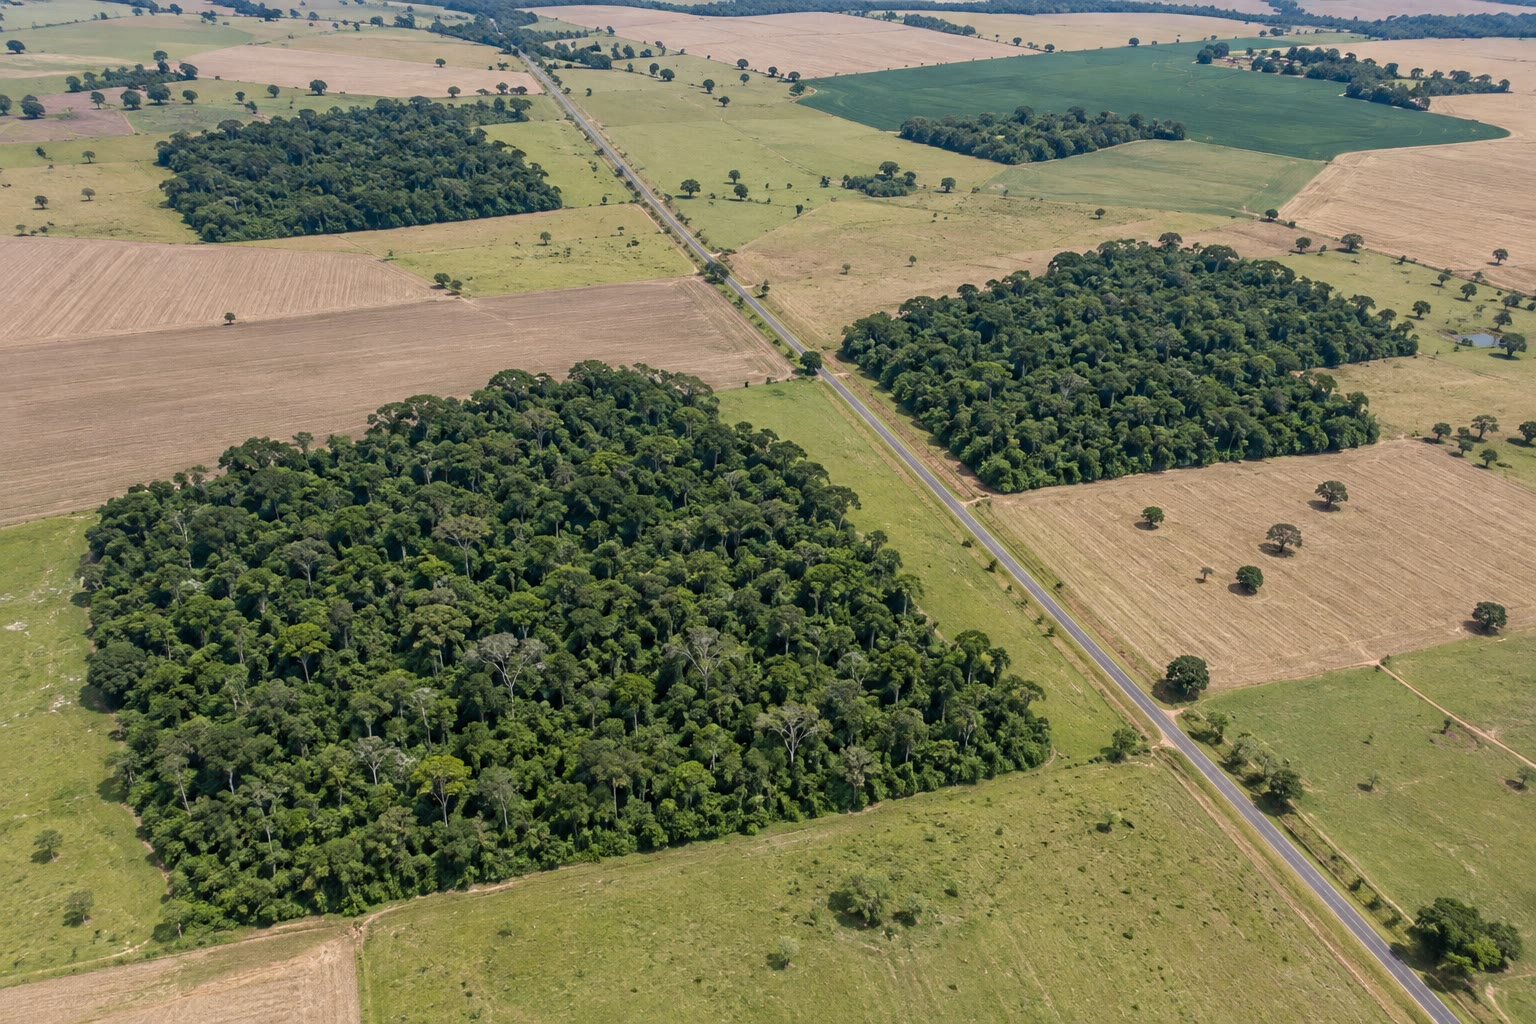
\includegraphics[width=0.6\linewidth]{images/book5/ai/b5-27-forest-fragments.jpg}

{\small Des fragments de forêt dans des terres cultivées, vus du ciel~:
chaque île abrite une population plus petite que ne l'était l'ensemble,
bordée d'une zone que les espèces d'intérieur ne peuvent employer, et
séparée par des champs que les espèces forestières ne peuvent traverser.}
\end{omfigure}

\section{Prévoir et prévenir}

\begin{method}[L'analyse de viabilité des populations]\label{met:b3:conservation-biology:pva}
\index{analyse de viabilité des populations}\index{quasi-extinction}
Pour estimer le risque d'extinction d'une population et ce qui le
réduirait~: (1) bâtir un modèle de sa dynamique --- une matrice de
survies et de fécondités par âge ou par stade, comme dans la démographie
du volume de deuxième année, estimée sur des individus marqués pendant
plusieurs années~; (2) ajouter la stochasticité --- démographique, en
tirant au hasard le sort de chaque individu, et environnementale, en
tirant les taux de chaque année dans leur variance observée, avec des
catastrophes occasionnelles~; (3) ajouter la dépendance à la densité et
le déclin génétique dû à la consanguinité là où les données le
permettent~; (4) simuler des milliers de trajectoires depuis l'effectif
actuel sur l'horizon qui intéresse et noter la fraction qui passe
au-dessous d'un seuil de \emph{quasi-extinction} (une taille dont on
juge le rétablissement impossible)~; (5) faire varier les entrées ---
survie des adultes, survie des jeunes, aire d'habitat, translocation de
dix animaux --- et voir quel changement réduit le plus le risque~: c'est
là qu'il faut porter l'effort. La sortie est une probabilité entourée
d'une large incertitude, non une prédiction~; sa valeur est
comparative, et elle a montré maintes fois que c'est la survie des
adultes, non la fécondité, qui est le levier chez les espèces à longue
vie, et c'est pourquoi les palangres tuent les populations d'albatros,
qui pondent un œuf tous les deux ans, plus vite qu'aucune perte de nids.
\end{method}

\begin{proposition}[Le temps jusqu'à l'extinction]\label{prop:b3:conservation-biology:time}
\index{temps jusqu'à l'extinction}
Pour une population qui fluctue parce que l'environnement fluctue, de
taux de croissance moyen $\bar r$ proche de zéro et de variance
$\sigma^{2}$ du taux de croissance annuel, le logarithme de la taille de
population suit une marche au hasard avec dérive, et le temps attendu
jusqu'à l'extinction depuis une taille $N$ ne croît que comme le
\emph{logarithme} de $N$ quand $\bar r < 0$ --- doubler la population
ajoute un nombre fixe d'années --- et comme une \emph{puissance} de $N$
quand $\bar r > 0$, d'exposant $2\bar r/\sigma^{2} - 1$~; sous la seule
\omterm{def:b3:conservation-biology:small}{stochasticité démographique} il croît \emph{exponentiellement} avec $N$,
de sorte qu'une population à l'abri du hasard démographique à cent
individus peut encore être perdue à la variance environnementale à dix
mille. La conséquence pratique est que réduire la variance de la
croissance d'une population --- l'amortir contre les mauvaises années
par plus d'habitat, plus de sites, un régime plus large --- peut faire
plus pour sa persistance que relever sa moyenne.
\end{proposition}
\admitted

\begin{omfigure}
\begin{tikzpicture}
\begin{semilogyaxis}[
  width=0.62\linewidth, height=5.4cm,
  axis x line=bottom, axis y line=left,
  xmin=0, xmax=50, ymin=1, ymax=3000,
  xlabel={années}, ylabel={effectif de la population},
  xlabel style={font=\small, at={(axis description cs:0.5,-0.12)}, anchor=north}, ylabel style={font=\small},
  tick label style={font=\small}, xtick={0,10,20,30,40,50}, ytick={1,10,100,1000}, yticklabels={1,10,100,1000},
  clip=false,
]
\addplot[thick, omDef] coordinates {(0,200) (2,240) (4,190) (6,260) (8,300) (10,220) (12,180) (14,250) (16,330) (18,280) (20,350) (22,300) (24,260) (26,340) (28,420) (30,380) (32,450) (34,400) (36,520) (38,480) (40,560) (42,500) (44,600) (46,650) (48,610) (50,700)};
\addplot[thick, omThm] coordinates {(0,200) (2,150) (4,180) (6,120) (8,90) (10,110) (12,70) (14,50) (16,60) (18,35) (20,40) (22,25) (24,18) (26,22) (28,12) (30,8) (32,9) (34,5) (36,3) (38,2) (40,1)};
\addplot[thick, omMeth!70!black] coordinates {(0,200) (2,210) (4,170) (6,200) (8,140) (10,160) (12,120) (14,140) (16,90) (18,110) (20,80) (22,95) (24,60) (26,75) (28,50) (30,55) (32,40) (34,45) (36,30) (38,35) (40,28) (42,30) (44,22) (46,25) (48,20) (50,22)};
\draw[dashed, gray] (axis cs:0,20) -- (axis cs:50,20); \node[font=\scriptsize, gray, anchor=north east] at (axis cs:49,18) {seuil de quasi-extinction};
\node[font=\scriptsize, omDef, anchor=west] at (axis cs:50.5,700) {$\bar r > 0$~: persiste};
\node[font=\scriptsize, omMeth!70!black, anchor=west] at (axis cs:50.5,22) {$\bar r \approx 0$~: dérive vers le bas};
\node[font=\scriptsize, omThm, anchor=west] at (axis cs:40.5,1.3) {$\bar r < 0$~: disparue en 40 ans};
\end{semilogyaxis}
\end{tikzpicture}

{\small Trois trajectoires simulées à partir des mêmes deux cents
animaux, qui ne diffèrent que par le taux de croissance moyen~; une
analyse de viabilité en fait tourner des milliers et compte combien
franchissent le seuil. C'est la variance d'une année à l'autre qui fait
même du cas médian un pari.}
\end{omfigure}

\begin{definition}[Les outils]\label{def:b3:conservation-biology:tools}
\index{liste rouge de l'UICN}\index{espèce envahissante}\index{conservation ex situ}\index{élevage en captivité}\index{réintroduction}\index{réensauvagement}\index{cascade trophique}
La \emph{liste rouge de l'UICN} classe les espèces selon des critères
quantitatifs~: un déclin de \qty{30}{\%}, \qty{50}{\%} ou \qty{80}{\%}
en dix ans ou trois générations, une aire de répartition au-dessous de
\qty{20000}{}, \qty{5000}{} ou \qty{100}{km^2}, une population
au-dessous de \qty{10000}{}, \qty{2500}{} ou \qty{250}{} individus
matures, ou une probabilité d'extinction modélisée, rangent une espèce
comme vulnérable, en danger ou en danger critique~; un quart des
mammifères et un huitième des oiseaux y entrent. Les causes sont la
perte d'habitat d'abord, puis la surexploitation, les \emph{espèces
envahissantes} (prédateurs et concurrents portés vers des îles dont les
espèces ne les avaient jamais rencontrés~: rats, chats et hermines ont
pris la plupart des oiseaux de Nouvelle-Zélande, une seule espèce de
serpent brun arboricole la plupart de ceux de Guam), la pollution et le
changement climatique. Les réponses~: des aires protégées couvrant un
sixième des terres~; le contrôle ou l'éradication des envahisseurs (cent
cinquante îles débarrassées des rats)~; la conservation \emph{ex situ}
--- des banques de graines qui gardent un million d'accessions dans un
coffre du pergélisol arctique, des embryons congelés, et l'\emph{élevage
en captivité} à généalogies gérées pour minimiser l'apparentement, qui a
ramené le condor de Californie de vingt-deux oiseaux en 1987 et le furet
à pieds noirs de dix-huit~; la \emph{réintroduction}, qui réussit
environ une fois sur trois et plus souvent quand la cause de la perte
initiale a été levée~; et le \emph{réensauvagement}, le retour des
grands animaux et des processus qu'ils entraînent --- les loups de
Yellowstone, dont la prédation et la peur qu'elle inspire ont éloigné
les wapitis des berges et laissé revenir saule, tremble, castor et
oiseaux chanteurs, une \emph{cascade trophique} qui court d'un carnivore
à la forme d'une rivière.
\end{definition}

\begin{omfigure}
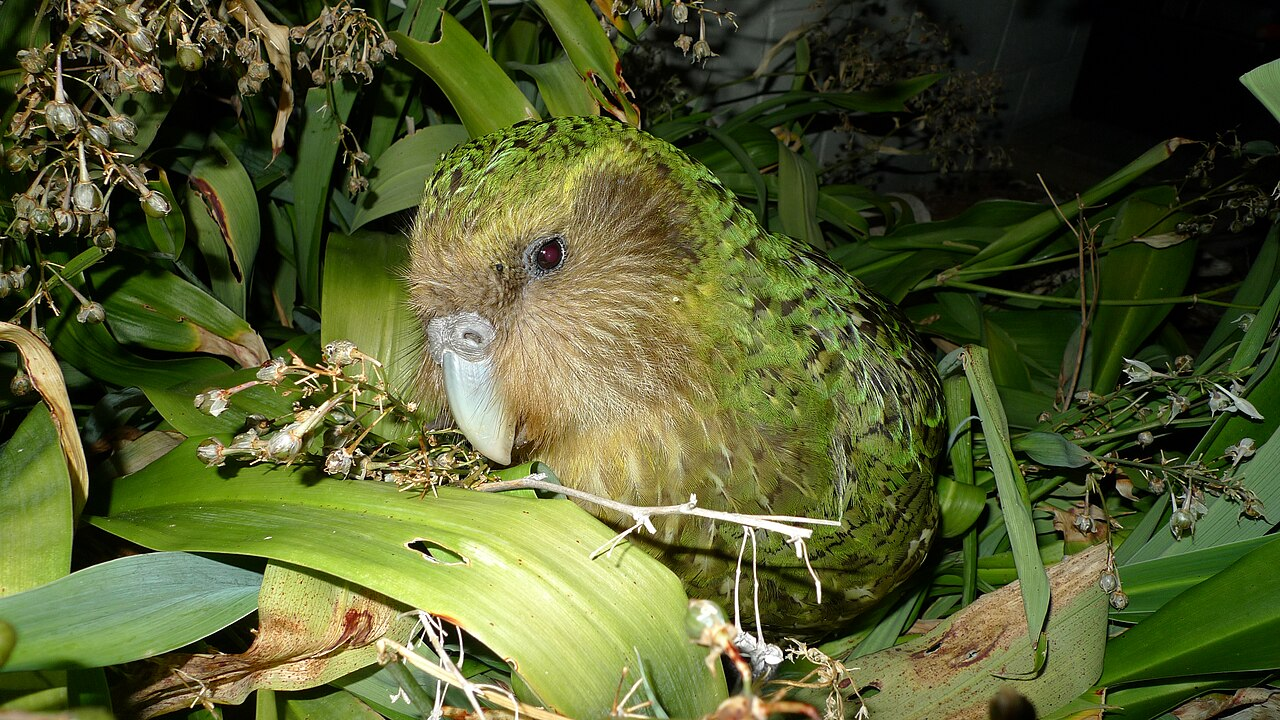
\includegraphics[width=0.46\linewidth]{images/book5/kakapo-sirocco.jpg}\hspace{0.04\linewidth}
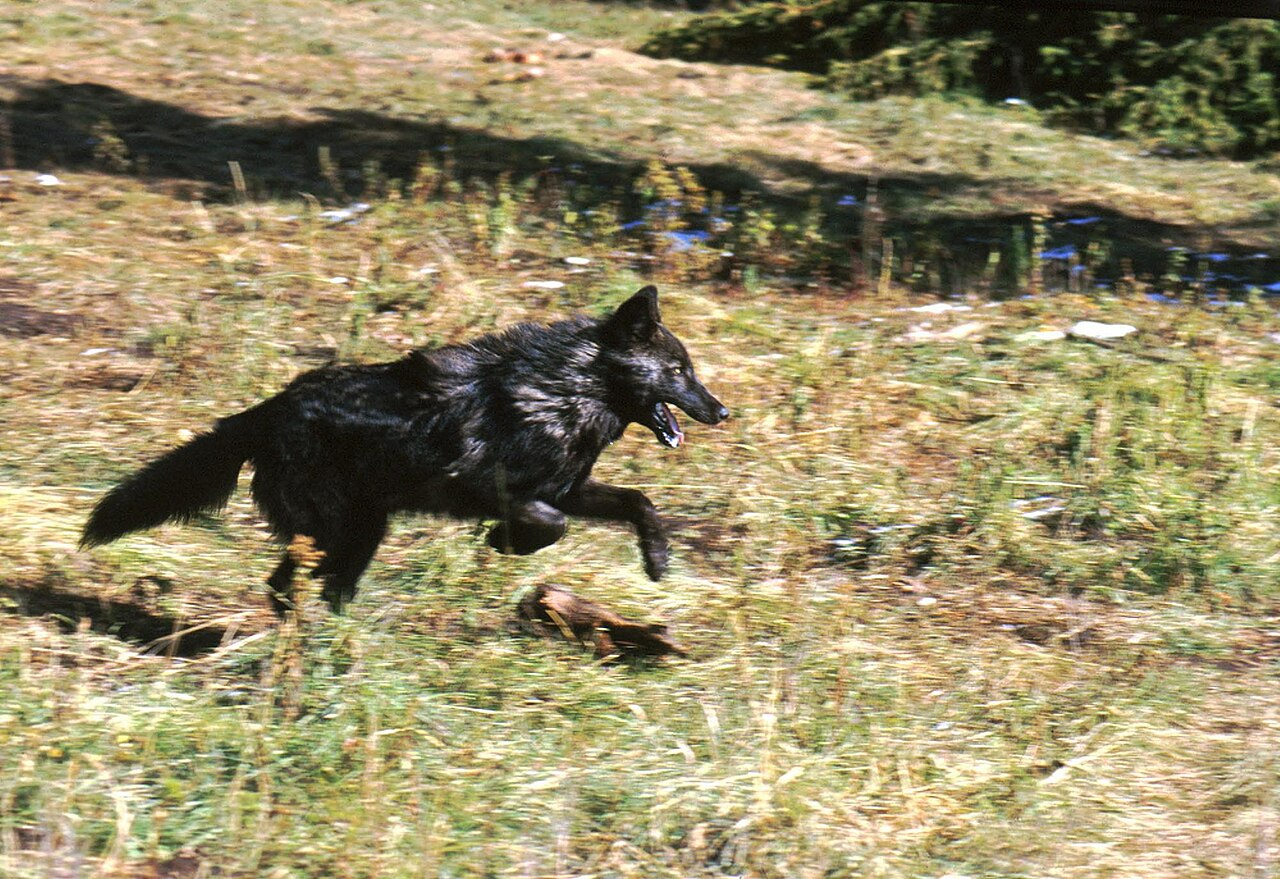
\includegraphics[width=0.46\linewidth]{images/book5/yellowstone-wolves-1996.jpg}

{\small À gauche~: Sirocco, un kakapo --- l'un des cinquante et un
survivants de 1995, aujourd'hui l'un de quelque deux cent cinquante,
tous nommés et suivis sur des îles sans prédateurs (photographie~:
Department of Conservation, Nouvelle-Zélande, CC BY 2.0). À droite~: des
loups à Yellowstone en 1996, le premier hiver après leur \omterm{def:b3:conservation-biology:tools}{réintroduction}
(photographie~: National Park Service, domaine public).}
\end{omfigure}

\begin{example}[Trois rétablissements]\label{ex:b3:conservation-biology:recoveries}
Le kakapo~: cinquante et un oiseaux en 1995, tous déplacés sur des îles
débarrassées de leurs prédateurs~; chaque oiseau porte un émetteur,
chaque nid est surveillé par caméra, les poussins sont élevés à la main
quand une mère faiblit, les mâles sont nourris pour les amener en
condition de reproduction les années où les rimus fructifient, et la
généalogie est gérée pour garder dans la population les gènes rares du
dernier mâle du Fiordland~; le génome de chaque kakapo a été séquencé.
Deux cent cinquante aujourd'hui, et un $N_{e}$ que les génomes situent
près de cent. La grue blanche d'Amérique~: quinze oiseaux en 1941, un
seul vol migrateur, élevée en captivité à partir d'œufs pris dans des
nids sauvages, à qui l'on a appris de nouvelles routes de migration
derrière des ULM, et qui compte aujourd'hui quelque huit cents
individus. La baleine à bosse~: chassée jusqu'à quelques milliers,
protégée en 1966, et désormais au-delà de cent mille, une hausse
d'environ \qty{8}{\%} par an qui montre ce que fait un animal à longue
vie quand on lève l'unique cause de son déclin. Chaque rétablissement a
coûté des dizaines de millions et des décennies~; l'arithmétique du
chapitre dit pourquoi l'effort devait être consenti avant que les
effectifs n'atteignent le vortex, et pourquoi il revenait moins cher que
tout sauvetage ultérieur.
\end{example}

\begin{omfigure}
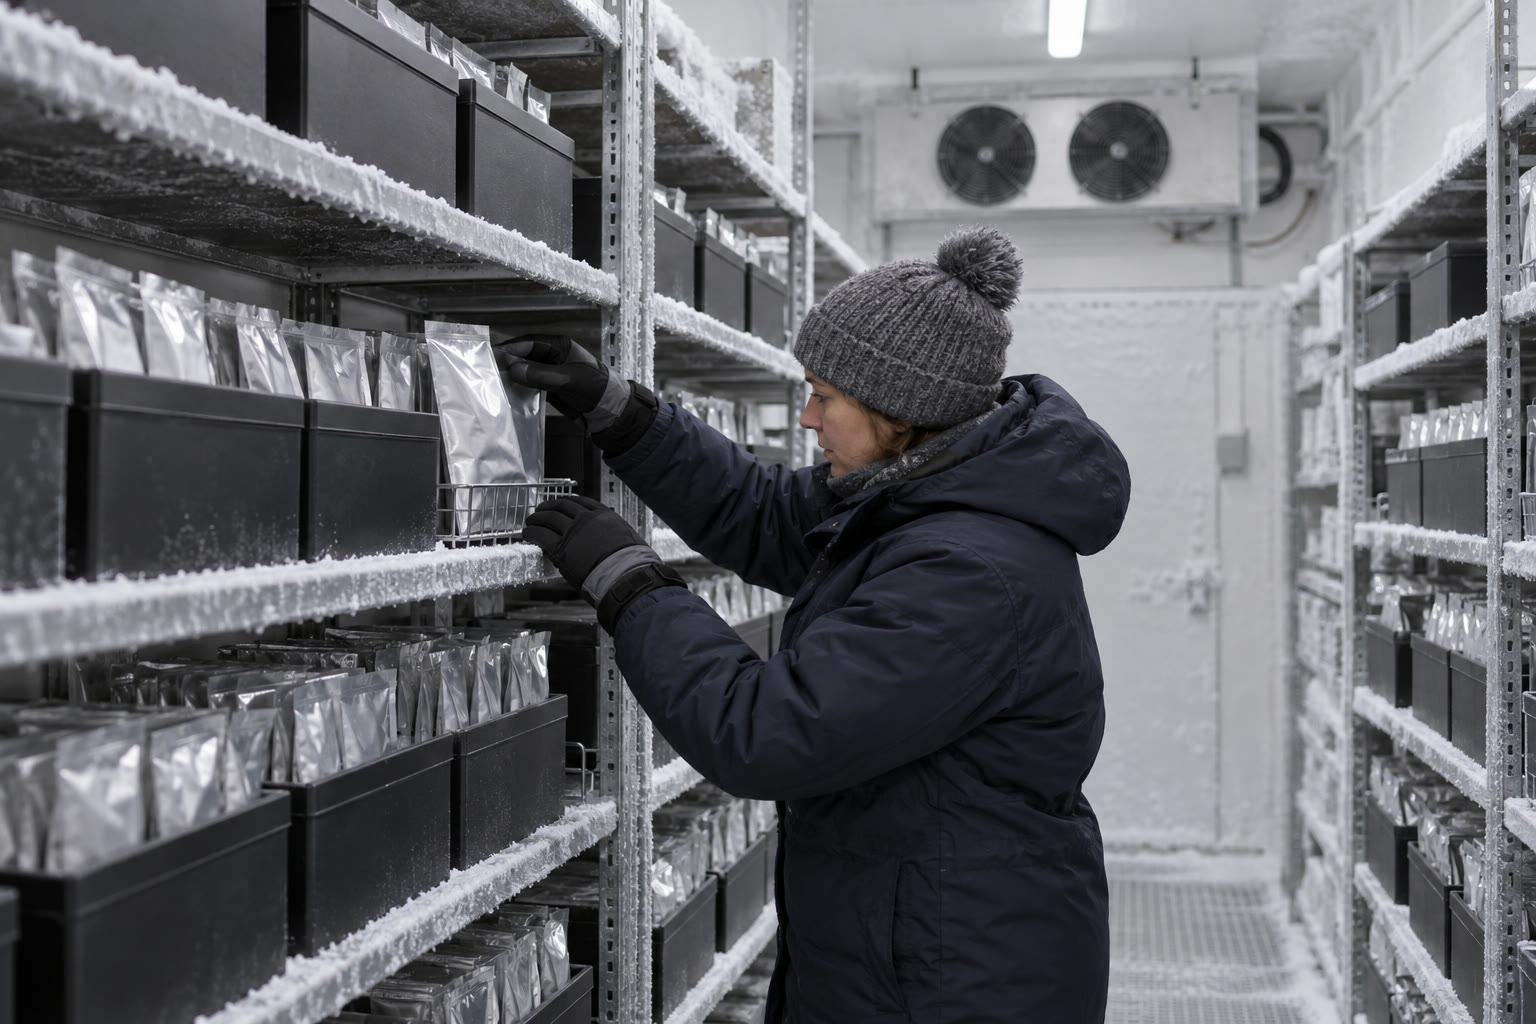
\includegraphics[width=0.56\linewidth]{images/book5/ai/b5-27-seed-vault.jpg}

{\small Un coffre à graines dans le pergélisol~: les doubles d'un
million d'accessions de plantes cultivées et sauvages, tenues à
\qty{-18}{\celsius} contre la perte des collections dont elles viennent
--- la conservation comme assurance, à l'échelle du génome d'une espèce.}
\end{omfigure}

\begin{remark}[L'arithmétique de la préservation]\label{rem:b3:conservation-biology:remark}
Chaque chapitre de ce cours s'est achevé sur un nombre, et celui-ci
s'achève sur plusieurs~: une taille efficace, un \omterm{thm:b3:conservation-biology:ne}{coefficient de
consanguinité} qui monte de $1/2N_{e}$ par génération, un exposant $z$
qui change des hectares perdus en espèces perdues, une probabilité
d'extinction sur un siècle. Ils sont grossiers --- le recensement est
incertain, la variance est devinée, le modèle est une caricature --- et
ce sont eux qui changent un sentiment sur des oiseaux qui disparaissent
en une décision sur les cinquante hectares à acheter et les huit animaux
à déplacer. La biologie est la même que dans tout le reste du livre~:
dérive, sélection, démographie, comportement, dépendance d'une
population à son habitat et d'un habitat à ses populations. Ce qui est
neuf n'est que l'urgence, et le fait que l'expérience se fait une seule
fois, sans témoin, sur les espèces qui restent.
\end{remark}

\section{Exercices}

\begin{exercise}[$\star$]\label{exo:b3:conservation-biology:1}
Définir la \omterm{def:b3:conservation-biology:small}{stochasticité démographique}, la \omterm{def:b3:conservation-biology:small}{stochasticité
environnementale} et l'\omterm{def:b3:conservation-biology:small}{effet Allee}, et donner un exemple de chacun tiré
du chapitre.
\end{exercise}

\begin{exercise}[$\star$]\label{exo:b3:conservation-biology:2}
Qu'est-ce que la \omterm{thm:b3:conservation-biology:ne}{taille efficace de population}, et nommer trois traits
d'une population réelle qui la rendent plus petite que l'effectif
recensé.
\end{exercise}

\begin{exercise}[$\star$]\label{exo:b3:conservation-biology:3}
Énoncer la loi aire--espèces. Si $z = 0.25$, quelle fraction des espèces
un habitat garde-t-il après avoir perdu la moitié de son aire~? Les neuf
dixièmes~? Les quatre-vingt-dix-neuf centièmes~?
\end{exercise}

\begin{exercise}[$\star$]\label{exo:b3:conservation-biology:4}
Expliquer la règle 50/500, et ce contre quoi chaque nombre protège.
\end{exercise}

\begin{exercise}[$\star\star$]\label{exo:b3:conservation-biology:5}
Une harde de 200 éléphants de mer compte 8 mâles reproducteurs et 120
femelles reproductrices. Calculer $N_{e}$ et la perte d'hétérozygotie
par génération. Combien de générations pour en perdre le quart~?
\end{exercise}

\begin{exercise}[$\star\star$]\label{exo:b3:conservation-biology:6}
Une population a compté 1000, 1000, 20, 1000, 1000 sur cinq générations
successives. Calculer $N_{e}$ sur l'intervalle, et l'hétérozygotie
conservée, et comparer à un effectif constant de 1000.
\end{exercise}

\begin{exercise}[$\star\star$]\label{exo:b3:conservation-biology:7}
Vingt-cinq panthères de Floride avec $N_{e} \approx 10$~: consanguinité
accumulée en 5 générations~? Si la valeur sélective baisse de
\qty{5}{\%} par tranche de \qty{10}{\%} de $F$, de combien a-t-elle
baissé~? Que fait l'ajout de huit femelles non apparentées au $F$ de la
génération suivante~?
\end{exercise}

\begin{exercise}[$\star\star$]\label{exo:b3:conservation-biology:8}
Yellowstone~: 31 loups lâchés en 1995--96, environ 100 dans le parc en
2003. Estimer $r$~; combien y en aurait-il en 2020 si la croissance
s'était poursuivie, et pourquoi ne l'a-t-elle pas fait~?
\end{exercise}

\begin{exercise}[$\star\star$]\label{exo:b3:conservation-biology:9}
Classer selon les critères de l'UICN du chapitre~: (a) une grenouille
dont la population a chuté de \qty{60}{\%} en dix ans~; (b) une plante
de 180 individus matures~; (c) un poisson dont l'aire de répartition
fait \qty{3000}{km^2}~; (d) un oiseau de \num{30000} individus qui
décline de \qty{10}{\%} par décennie.
\end{exercise}

\begin{exercise}[$\star\star\star$]\label{exo:b3:conservation-biology:10}
Une population de $N$ couples produisant chacun, avec la probabilité
$1/2$, deux descendants survivants et sinon aucun (\omterm{def:b3:conservation-biology:small}{stochasticité
démographique}). Calculer la probabilité que toute la population échoue
en une génération pour $N = 2$, $5$, $10$, $20$, et commenter la façon
dont le risque démographique varie avec $N$.
\end{exercise}

\begin{exercise}[$\star\star\star$]\label{exo:b3:conservation-biology:11}
La loi aire--espèces avec $z = 0.25$, et une forêt coupée en 10
fragments isolés égaux. Comparer les espèces attendues dans un fragment
avec un dixième de l'originale, et argumenter pourquoi le total sur les
fragments n'est pas simplement l'originale --- qu'est-ce qui détermine
si les fragments réunis abritent plus ou moins d'espèces que le tout~?
\end{exercise}

\begin{exercise}[$\star\star\star$]\label{exo:b3:conservation-biology:12}
Pourquoi ajouter quelques migrants par génération ($m N_{e} \approx 1$)
arrête-t-il largement la perte de variation dans une petite population,
et qu'en coûte-t-il à l'adaptation locale~? Argumenter par l'équilibre
entre la dérive, $1/2N_{e}$, et la fraction d'allèles remplacés par les
migrants, $m$.
\end{exercise}

\section{Problème~: cinquante et cinq cents}

\begin{problem}[{Problème du week-end --- un programme de rétablissement
en chiffres~: la taille efficace d'une population de perroquets sauvée et
sa consanguinité, un sauvetage génétique, les espèces que gardera une
forêt qui rétrécit, la croissance de loups réintroduits, et les
catégories et les coûts, pour finir sur $N_{e}$, la consanguinité après
dix générations et la fraction d'espèces conservées}]
\label{pb:b3:conservation-biology:1}
Données~: une population de perroquets de 60 adultes, 20 mâles et 40
femelles, tous reproducteurs~; temps de génération \qty{10}{yr}.
Histoire de la population sur les cinq dernières générations~: 500, 100,
60, 51, 60. Dépression de consanguinité~: la valeur sélective baisse de
\qty{6}{\%} par \qty{0.1}{} de $F$. Sauvetage~: 10 oiseaux non apparentés
ajoutés aux 60. Forêt~: \qty{2000}{km^2} réduits à \qty{300}{km^2},
$z = 0.25$~; 180 espèces aujourd'hui. Loups~: 31 lâchés, 100 huit ans
plus tard, capacité de charge du parc environ 120. Coût~: quatre
millions de dollars par an pour les perroquets.

\medskip
\noindent\textbf{Partie I --- La taille efficace.}
\begin{enumerate}
  \item $N_{e}$ d'après le sex-ratio des 60 actuels. Comparer à
        l'effectif recensé.
  \item $N_{e}$ en \omterm{thm:b3:conservation-biology:ne}{moyenne harmonique} sur les cinq générations de
        l'histoire. Quelle génération domine~?
  \item Consanguinité accumulée sur ces cinq générations, avec le
        $N_{e}$ en \omterm{thm:b3:conservation-biology:ne}{moyenne harmonique} (formule exacte et approximation
        linéaire).
  \item Valeur sélective perdue à cette consanguinité.
  \item Hétérozygotie conservée après les cinq générations, en fraction
        de l'originale.
  \item Si la population est désormais tenue à 60 avec le sex-ratio
        actuel, quel $F$ atteindra-t-elle en dix générations de plus, et
        quelle perte de valeur sélective~? Combien d'années cela fait-il~?
\end{enumerate}

\medskip
\noindent\textbf{Partie II --- Le sauvetage.}
\begin{enumerate}[resume]
  \item Dix oiseaux non apparentés rejoignent les 60. La fraction des
        allèles de la génération suivante qui vient des nouveaux venus
        vaut environ $10/70$~; le \omterm{thm:b3:conservation-biology:ne}{coefficient de consanguinité} des
        descendants d'un parent local et d'un nouveau venu vaut $0$.
        Estimer le $F$ moyen de la population à la génération suivante si
        les accouplements sont au hasard.
  \item Expliquer pourquoi $F$ baisse aussitôt mais que l'hétérozygotie
        ne monte qu'à mesure que les allèles des migrants se répandent,
        et pourquoi un second sauvetage peut être nécessaire.
  \item Pour atteindre $N_{e} = 500$ avec un sex-ratio équilibré, combien
        d'adultes faut-il~? À $r = \qty{0.05}{yr^{-1}}$ depuis 70
        oiseaux, combien d'années~?
  \item Le programme retire les œufs des mauvaises mères pour un élevage
        à la main, ce qui élève le nombre moyen de jeunes à l'envol par
        couple mais égalise les tailles de familles. Pourquoi égaliser
        les tailles de familles \emph{élève}-t-il $N_{e}$ au-dessus de
        l'effectif recensé (vers $2N$)~?
  \item Le dernier mâle d'une lignée méridionale distincte est stérile
        en nature. Proposer deux interventions et leur coût pour le pool
        génétique.
  \item À quatre millions de dollars par an pendant les 40 ans qu'il
        faut pour atteindre $N_{e} = 500$, coût total et coût par oiseau
        ajouté. Est-ce cher~? Comparé à quoi~?
\end{enumerate}

\medskip
\noindent\textbf{Partie III --- La forêt.}
\begin{enumerate}[resume]
  \item Fraction des espèces que la forêt gardera à \qty{300}{km^2}~;
        nombre d'espèces attendu, et dette d'extinction (les espèces
        présentes aujourd'hui qui seront perdues).
  \item Si au lieu de cela les \qty{300}{km^2} étaient trois fragments
        isolés de \qty{100}{km^2}, espèces par fragment~; total si les
        fragments abritaient des espèces entièrement différentes~; total
        s'ils abritaient les mêmes. Qu'est-ce qui décide~?
  \item Un corridor de \qty{20}{km^2} relie les trois fragments. Les
        traiter comme une seule aire de \qty{320}{km^2}~: espèces
        attendues. Comparer au cas des espèces identiques de la
        question~14.
  \item Le plus grand prédateur de la forêt a besoin de \qty{50}{km^2}
        par couple et d'un $N_{e}$ de 50 pour persister. Les
        \qty{300}{km^2} entiers peuvent-ils l'abriter~? Un fragment~? Que
        dit cela de l'aire face au nombre d'espèces comme critère~?
  \item Estimer le temps que met la dette d'extinction à se payer si les
        espèces perdues ont des populations qui déclinent de \qty{3}{\%}
        par an de 200 jusqu'à un seuil de quasi-extinction de 10.
  \item Pourquoi la loi aire--espèces sous-estime-t-elle la perte quand
        la fragmentation ajoute des \omterm{prop:b3:conservation-biology:area}{effets de lisière}, et la
        surestime-t-elle quand les terres alentour sont en partie
        utilisables~?
\end{enumerate}

\medskip
\noindent\textbf{Partie IV --- Loups et listes.}
\begin{enumerate}[resume]
  \item Les loups~: $r$ de $31 \to 100$ en 8 ans, et le temps de
        doublement.
  \item Croissance logistique vers $K = 120$~: population après 8 ans
        sous une croissance logistique plutôt qu'exponentielle, en
        partant de 31 avec le $r$ de la question~19 (employer
        $N(t) = K/[1 + (K/N_{0} -
        1)\mathrm{e}^{-rt}]$). Laquelle s'accorde le mieux aux 100
        observés, et que dit cela de la dépendance à la densité des
        premières années~?
  \item Les wapitis étaient \num{17000} en 1995 et \num{4000} en 2015.
        Taux de déclin annuel moyen. Quelle part en expliquent des loups
        mangeant \num{20} wapitis chacun par an, à 100 loups~?
  \item Classer le perroquet (60 individus matures) et le prédateur de
        la forêt d'avant le sauvetage selon les critères de l'UICN.
  \item La tourte voyageuse~: cinq milliards en 1800, éteinte en 1914. Si
        le déclin a été exponentiel de 1870, où elles se comptaient
        encore en milliards, à un seul oiseau en 1914, quel taux annuel
        cela implique-t-il~? Pourquoi l'\omterm{def:b3:conservation-biology:small}{effet Allee} rend-il les dernières
        décennies plus rapides qu'une exponentielle~?
  \item Expliquer en un paragraphe pourquoi une AVP aurait dit que la
        tourte voyageuse était en sûreté en 1850, et ce qu'elle aurait
        manqué.
  \item Résumer~: le $N_{e}$ actuel (question~1), le $F$ après dix
        générations de plus à 60 (question~6), et la fraction d'espèces
        que garde la forêt rétrécie (question~13).
\end{enumerate}
\end{problem}
